\documentclass[11pt,a4paper]{article}

\usepackage[utf8]{inputenc}
\usepackage[T1]{fontenc}
\usepackage{lmodern}
\usepackage[margin=1in]{geometry}
\usepackage{amsmath,amssymb}
\usepackage{graphicx}
\usepackage{booktabs}
\usepackage{tabularx}
\usepackage{caption}
\usepackage{subcaption}
\usepackage{natbib}
\usepackage{hyperref}
\usepackage[capitalise,nameinlink]{cleveref}
\crefname{equation}{Equation}{Equations}
\Crefname{equation}{Equation}{Equations}
\usepackage{titlesec}

% Methodology subsections numbered 4a, 4b, 4c instead of 4.1, 4.2, 4.3
\renewcommand{\thesubsection}{\thesection\alph{subsection}}
\usepackage{xcolor}
\usepackage{array}
\usepackage{enumitem}
\usepackage{pdflscape}
\usepackage{tikz}
\usetikzlibrary{calc,positioning}
\usepackage{float}
\usepackage{placeins}

\hypersetup{colorlinks=true, linkcolor=black, citecolor=blue, urlcolor=blue}
\setlength{\parindent}{0pt}
\setlength{\parskip}{6pt}
\titlespacing*{\section}{0pt}{14pt}{6pt}
\titlespacing*{\subsection}{0pt}{10pt}{4pt}

\title{\vspace{-1cm}\bfseries Do Mobility Beliefs Reduce Support for Redistribution in Transition Economies?\\Evidence from LiTS IV with Fairness-Belief Moderation}
\author{Dovud Asadov\\\small Department of Economics, New Uzbekistan University\\\small\texttt{d.asadov@newuu.uz}}
\date{}

\begin{document}
\maketitle

% =====================================================================
\section{Introduction}

One of the most counterintuitive phenomena in political economy is that the majority of
citizens whose income is below mean rarely support redistribution, which is opposite of
the median-voter model by \citet{meltzer1981rational}. Empirical evidence also supports
that preference toward redistribution is weaker than the inequality level would suggest
\citep{hoy2021relatively, alesina2018intergenerational}. \citet{benabou2001social}
offered an explanation with the ``Prospect of Upward Mobility'' (POUM) hypothesis, which
stated that when individuals have a belief that their income and wealth would change in
the future, they do not support redistribution as it may impose higher taxes on them
later. Complementary to that, \citet{piketty1995social} found that families change their
belief based on their own mobility experiences, whereas \citet{hirschman1973changing}
found a ``tunnel effect'' in which observing the upward mobility of others increases
tolerance for current inequality. Subsequent work shows that fairness beliefs also shape
redistribution demand \citep{alesina2005fairness, benabou2006belief,
alesina2018intergenerational}.

Based on the literature review there are three important limitations. First, the POUM
mechanism has been tested mostly on the United States \citep{alesina2005preferences} or
on a single transition country in the 1990s \citep{ravallion2000wants}. Although
performed at multi-country level by \citet{cojocaru2014prospects}, it is conducted prior
to the wave of reforms that began in 2010, assumes a dichotomy between the EU and
non-EU, and mixes up retrospective and prospective views. Second, the existence of a
POUM effect has not yet been tested in conjunction with individuals' belief that their
effort is not rewarded, which is clearly predicted by theory \citep{alesina2005fairness,
benabou2006belief}. Third, the prior literature has not tried the ten-step wealth
ladder, which provides a continuous expected mobility measure that compares the mobility
of individuals with very different incomes.

Moreover, complementary experiments used true information about people's inequality and
social mobility to show that beliefs causally shape redistribution demand
\citep{kuziemko2015elastic, karadja2017richer, roth2018expected, stantcheva2021perceptions}.
Whether the same mapping holds in post-socialist settings remains unclear
\citep{grosfeld2010comparing}.

This paper presents the first systematic evaluation of POUM on the LiTS IV (2022--23).
My four contributions are as follows: (i) I separate out retrospective, prospective and
``ladder-implied'' mobility beliefs and estimate their differential association to two
measures of attitudinal redistribution, (ii) I introduce the fairness-belief moderator,
based on the survey question ``What is the most important factor for success'', which
was not used in previous similar European studies \citep{alesina2005fairness,
alesina2018intergenerational}, (iii) I provide a joint specification that separates the
generalised-optimism channel of attitudinal items from the self-interest channel of
ladder-based items, and (iv) I take advantage of the cross-country variation across the
37 economies, including Central Asia and the Caucasus, which has been absent in previous
similar European studies \citep{alesina2005fairness, alesina2018intergenerational}.


% =====================================================================
\section{Objectives}

The purpose of this study is to estimate whether and how beliefs about upward income
mobility shape support for income redistribution across the 37 economies of the Life in
Transition Survey IV, and to decompose that relationship into a \emph{self-interest}
channel operating through respondents' own ladder positions and trajectories
\citep{benabou2001social} and a \emph{generalised-optimism} channel operating through
attitudinal mobility items \citep{hirschman1973changing, benabou2006belief,
alesina2018intergenerational}, allowing fairness beliefs to moderate both
\citep{alesina2005fairness}. The study pursues three specific objectives. First, it
estimates the partial association between six mobility-belief measures (attitudinal
items on parents-comparison, four-year retrospective, and prospective children, plus
three ladder-based measures of current, expected, and realised four-year ladder
mobility) and two redistribution outcomes, using OLS with country fixed effects and
country-clustered standard errors. Second, it disentangles the self-interest and
generalised-optimism channels through a joint ``horse-race'' specification placing
representative mobility measures on the right-hand side simultaneously, following the
channel-decomposition logic in \citet{alesina2018intergenerational,
stantcheva2021perceptions}. Third, it examines fairness-belief heterogeneity by
interacting each mobility variable with two indicators: belief that effort drives
success, and belief that political connections or breaking the law (i.e.\ injustice)
drive success. Region, cohort, and ladder-position splits are reported as exploratory
robustness checks rather than as a separate objective.


% =====================================================================
\section{Research Questions and Hypotheses}

\textbf{Research questions.}
\begin{enumerate}[leftmargin=28pt,itemsep=2pt,label=\textit{RQ\arabic*.}]
    \item Across the 37 economies, does a higher belief in upward mobility (past,
    current, or expected) predict support for income redistribution, conditional on
    demographics and country fixed effects?
    \item Is the mobility--redistribution association attributable to a
    \emph{self-interest} channel (operating through ladder-based measures) or to a
    \emph{generalised-optimism} channel (operating through attitudinal items)?
    \item Does the relationship depend on respondents' attribution of success to
    effort or to injustice?
\end{enumerate}

\textbf{Hypotheses.} Following \citet{benabou2001social, alesina2005preferences,
alesina2005fairness, alesina2018intergenerational, hirschman1973changing}:
\begin{itemize}[leftmargin=18pt,itemsep=2pt]
    \item[$H_{1}$:] \emph{Dual-channel mobility effect.} \emph{Ladder-based} mobility
    measures, capturing self-interested POUM, predict weaker redistribution demand
    ($\beta<0$). \emph{Attitudinal} mobility measures, capturing generalised optimism,
    predict stronger redistribution support ($\beta>0$).
    \item[$H_{2}$:] \emph{Asymmetric fairness moderation.} Belief that effort drives
    success steepens the channel-specific slope, while belief that injustice drives
    success attenuates or reverses it. Redistribution then becomes a fairness-correcting
    demand independent of own prospects.
    \item[$H_{3}$:] \emph{Behavioural consistency.} Sign and significance patterns are
    reproduced when the dependent variable is the binary willingness-to-pay outcome.
\end{itemize}

% =====================================================================
\section{Methodology}

\subsection{Data Collection Procedures}

Data are drawn from the Life in Transition Survey IV (LiTS IV), conducted jointly by
the EBRD and the World Bank between October 2022 and July 2023 \citep{ebrd2024lits}.
The survey covers 37 economies (33 EBRD countries of operation plus four comparators:
Czechia, Estonia, Germany, and Greece) with 37{,}478 face-to-face interviews. Sampling
proceeds via probability-proportional-to-size primary sampling units within
region\,$\times$\,urban/rural strata, random-walk household selection, and Kish-grid
selection of two adults per household (a knowledgeable respondent for socio-economic
items and a random primary respondent for attitudinal items). Population-scaled
weights \texttt{weight\_pop} are provided.
\emph{Variables.} Primary outcome: Q4.01f, 1--5 Likert agreement that ``the gap between
rich and poor should be reduced'' (pro-redistribution coded). Secondary outcome: Q4.05e,
a binary willingness to pay more taxes for poverty reduction. Mobility beliefs are six
measures: Q4.01b (vs.\ parents), Q4.01c (four-year retrospective), Q4.01e (prospective
children), Q2.35 (current ladder), Q2.37$-$Q2.35 (expected four-year mobility), and
Q2.35$-$Q2.36 (realised four-year mobility) \citep{cantril1965pattern, deaton2008income}.
Fairness moderators are binary indicators built from Q4.06 (effort $=1$; injustice
$\in\{3,4\}$). Controls: age, age$^2$, female, tertiary, married, urban, and log
monthly household income.

% =====================================================================
\subsection{Validation of Findings}

Five strategies stress-test the main finding. (i) \emph{Multiple operationalisations}:
six mobility measures and two redistribution outcomes, where concordant signs across
them strengthen inference (\cref{tab:main}). (ii) \emph{Population-weighted WLS}
(\cref{tab:weighted}) re-estimates the main specification using \texttt{weight\_pop} to
recover population-representative coefficients. (iii) \emph{Ordered-logit re-estimation}
(\cref{tab:ologit}) treats the 1--5 Likert outcome as ordinal rather than continuous
\citep{wooldridge2010econometric}. (iv) \emph{Joint horse-race regression}
(\cref{tab:joint}) places all four representative mobility variables on the right-hand
side simultaneously, separating the broad-optimism and self-interest channels.
(v) \emph{Triangulation}: signs and magnitudes are compared with
\citet{alesina2005preferences, ravallion2000wants, cojocaru2014prospects,
alesina2018intergenerational}. Sub-sample heterogeneity by ladder position, age cohort
(pre-/post-1980), and five-region splits is reported as exploratory
\citep{alesina2007goodbye, giuliano2014growing}.

% =====================================================================
\subsection{Data Analysis}

The base specification is OLS with country fixed effects and country-clustered
standard errors \citep{cameron2015practitioner, abadie2023should}:
\begin{equation}
\widetilde{R}_{ic} \;=\; \alpha + \beta\,\widetilde{M}_{ic} + \gamma'\,X_{ic}
+ \delta_{c} + \varepsilon_{ic},
\label{eq:base}
\end{equation}
where $\widetilde{R}_{ic}$ is standardised redistribution support, $\widetilde{M}_{ic}$
is one of the six standardised mobility-belief variables, $X_{ic}$ is the control
vector, and $\delta_{c}$ is a country fixed effect. Standardising both sides allows
coefficients to be read in within-country standard-deviation units
\citep{alesina2018intergenerational}. To test the dual-channel hypothesis $H_{1}$
(RQ2), four representative measures enter \cref{eq:base} simultaneously, isolating
each channel's marginal contribution \citep{stantcheva2021perceptions}. To test
$H_{2}$, I add a fairness interaction:
\begin{equation}
\widetilde{R}_{ic} \;=\; \alpha + \beta\,\widetilde{M}_{ic} + \theta\,F_{ic}
+ \pi\,(\widetilde{M}_{ic}{\times}F_{ic}) + \gamma'\,X_{ic} + \delta_{c}
+ \varepsilon_{ic}.
\label{eq:int}
\end{equation}
After listwise deletion the analytical sample is $N{\approx}28{,}000$ across 37
countries (income availability reduces $N$ from $35{,}766$). Analyses use Python~3.12
(\texttt{pandas}, \texttt{statsmodels}, \texttt{pyreadstat}) and are reproducible from
the public \texttt{.dta} file via the scripts in \texttt{analysis/}. Identification
rests on selection-on-observables, so estimates are interpreted as conditional
correlations rather than causal effects \citep{benabou2006belief}.



% =====================================================================
\section{Discussion}

Estimates from \cref{eq:base} support the dual-channel hypothesis $H_{1}$
(\cref{tab:main}, with the country-level pattern in \cref{fig:country}). The
attitudinal arm: mobility items load \emph{positively} on redistribution support
($\beta=+0.121$, $p<0.001$ for the parents-comparison item, and $\beta=+0.098$, $p<0.01$
for the prospective ``children will have a better life'' item), consistent with the
generalised-optimism prediction. The self-interest (POUM) arm: ladder-based measures
load negatively. Current ladder position ($\beta=-0.085$, $p<0.001$) and realised
four-year ladder gain ($\beta=-0.049$, $p<0.001$) are both significantly negative, while
expected ladder mobility is insignificant ($\beta=-0.015$, $p=0.24$).

\begin{figure}[H]
\centering
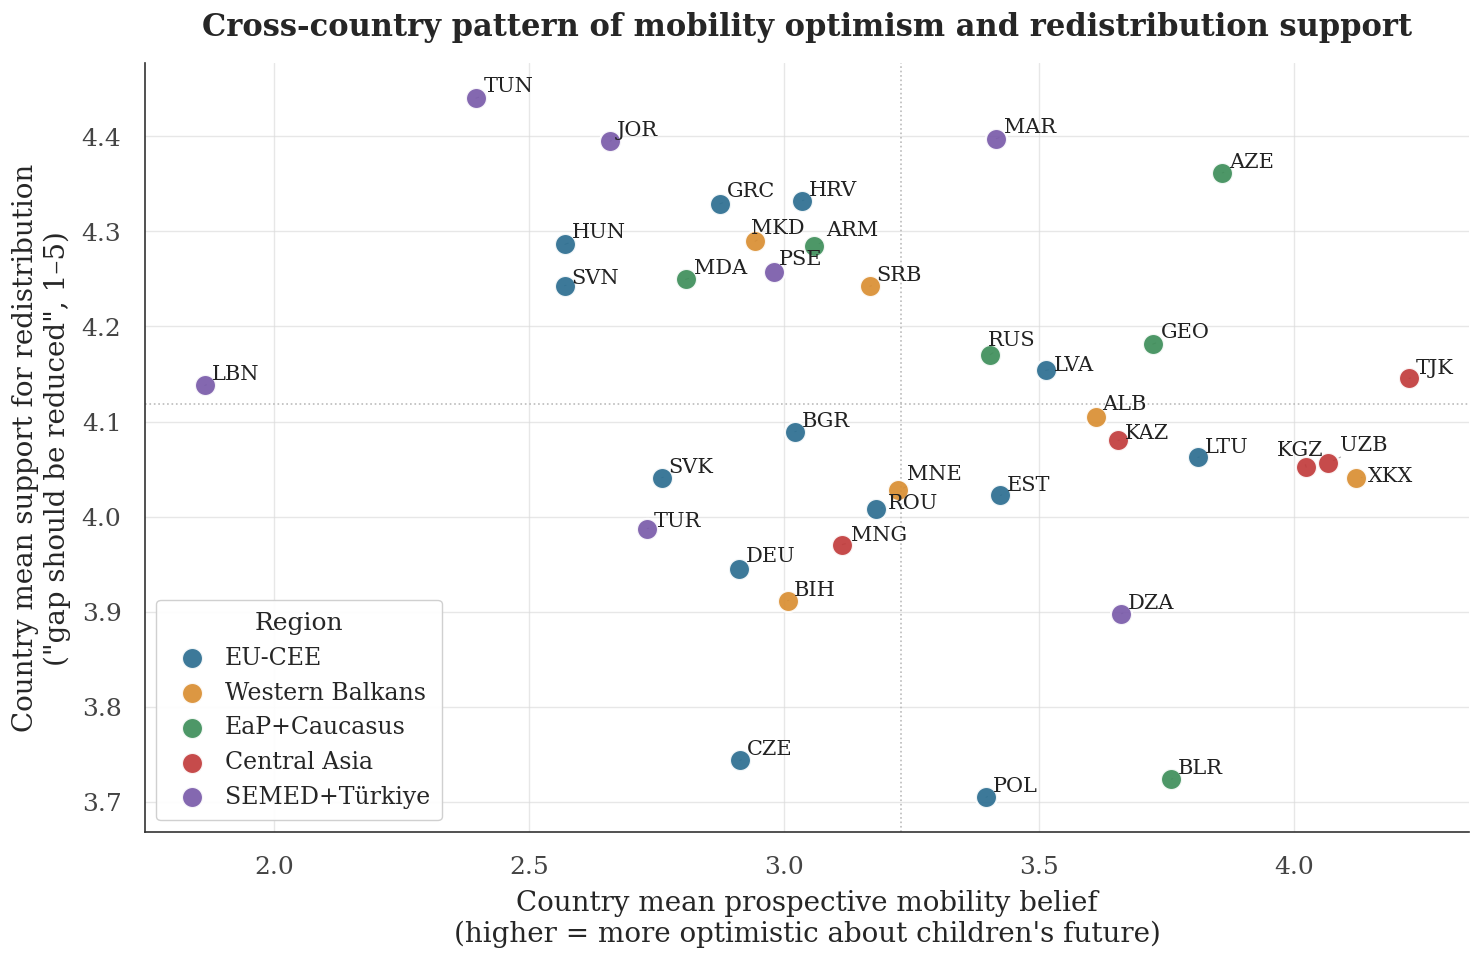
\includegraphics[width=0.82\textwidth]{output/fig_country_means.png}
\caption{Country-level means of redistribution support (Q4.01f) versus prospective
mobility (Q4.01e), LiTS~IV. Each dot is one of 37 economies, colour denotes the
five-region grouping, and dotted lines mark the sample means.}
\label{fig:country}
\end{figure}

The \emph{joint horse-race} regression in \cref{tab:joint} addresses RQ2 directly
and sharpens the channel decomposition. With all four representative mobility variables
on the right-hand side simultaneously, both ladder-based measures intensify and turn
unambiguously POUM-consistent: current ladder $\beta=-0.128$ ($p<0.001$) and
\emph{expected} ladder mobility $\beta=-0.057$ ($p<0.001$). The two attitudinal items
remain positive ($\beta_{\text{parents}}=+0.126$, $\beta_{\text{kids}}=+0.083$, both
$p<0.01$). The two arms of $H_{1}$ are therefore jointly supported. The
contrast is the central empirical pivot of the paper: ladder-based mobility captures the
self-interested POUM channel posited by \citet{benabou2001social}, whereas attitudinal
items load on a generalised pro-social optimism that is correlated with, but
analytically distinct from, expected income trajectories
\citep{alesina2018intergenerational, stantcheva2021perceptions}. Without separating
the two, the POUM effect is masked.

The fairness-belief interactions (\cref{tab:int}, \cref{fig:pred}) deliver the slope
asymmetry predicted by $H_{2}$. For prospective mobility, the \emph{effort}
interaction is positive ($\pi=+0.069$, $p<0.01$), and effort-believers steepen the
attitudinal slope. The \emph{injustice} interaction is negative ($\pi=-0.077$,
$p<0.001$), flattening and at the margin reversing it. For expected
ladder mobility, the injustice interaction is marginally significant
($\pi=-0.028$, $p\approx0.10$), in the same direction.

\begin{figure}[H]
\centering
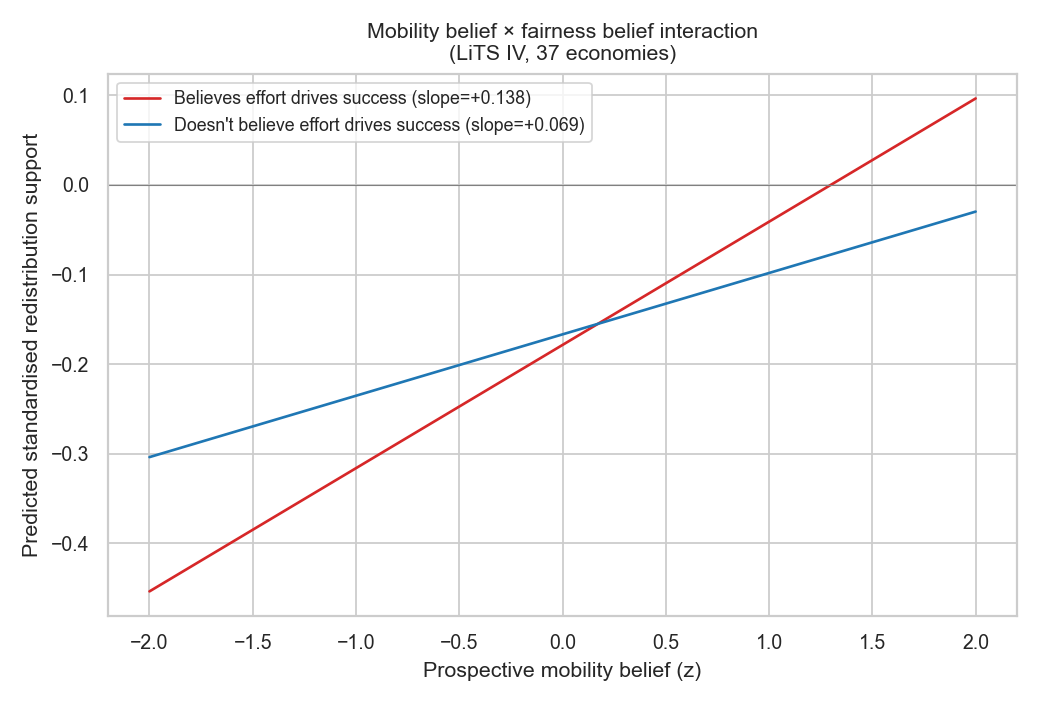
\includegraphics[width=0.78\textwidth]{output/fig_pred_interaction.png}
\caption{Predicted standardised redistribution support against prospective mobility
belief, by fairness belief. Country-fixed-effects OLS with country-clustered SEs, and
shaded bands are 95\% CIs. The slope is steeper for effort-believers and flatter for
those who do not endorse effort as the main driver of success (see \cref{tab:int}).}
\label{fig:pred}
\end{figure}

Exploratory heterogeneity tests confirm context-dependence. Across regions
(\cref{tab:regions}, \cref{fig:region}), prospective mobility loads most
strongly positive in Central Asia ($\beta=+0.456$, $p<0.001$), is essentially zero in
EU-CEE, and is positive but weaker in the Western Balkans, EaP+Caucasus, and
SEMED+T\"urkiye, a finer pattern than Cojocaru's binary EU/non-EU split. By age cohort
(\cref{tab:cohort}), the negative ladder-mobility coefficient is significant only
for respondents born before 1980 ($\beta=-0.028$, $p<0.05$) and disappears for the
post-Soviet cohort, consistent with the long-shadow channel in
\citet{alesina2007goodbye}. The ordered-logit re-estimation (\cref{tab:ologit})
preserves all signs and now lifts \emph{expected} ladder mobility to significance
($\beta=-0.039$, $p<0.01$), as does the population-weighted WLS specification
(\cref{tab:weighted}). $H_{3}$ finds partial support: on the binary WTP outcome
(\cref{tab:wtp}), all three mobility measures load \emph{positively}, mirroring
the attitudinal but not the ladder channel, consistent with the dual-channel framing.

\begin{figure}[H]
\centering
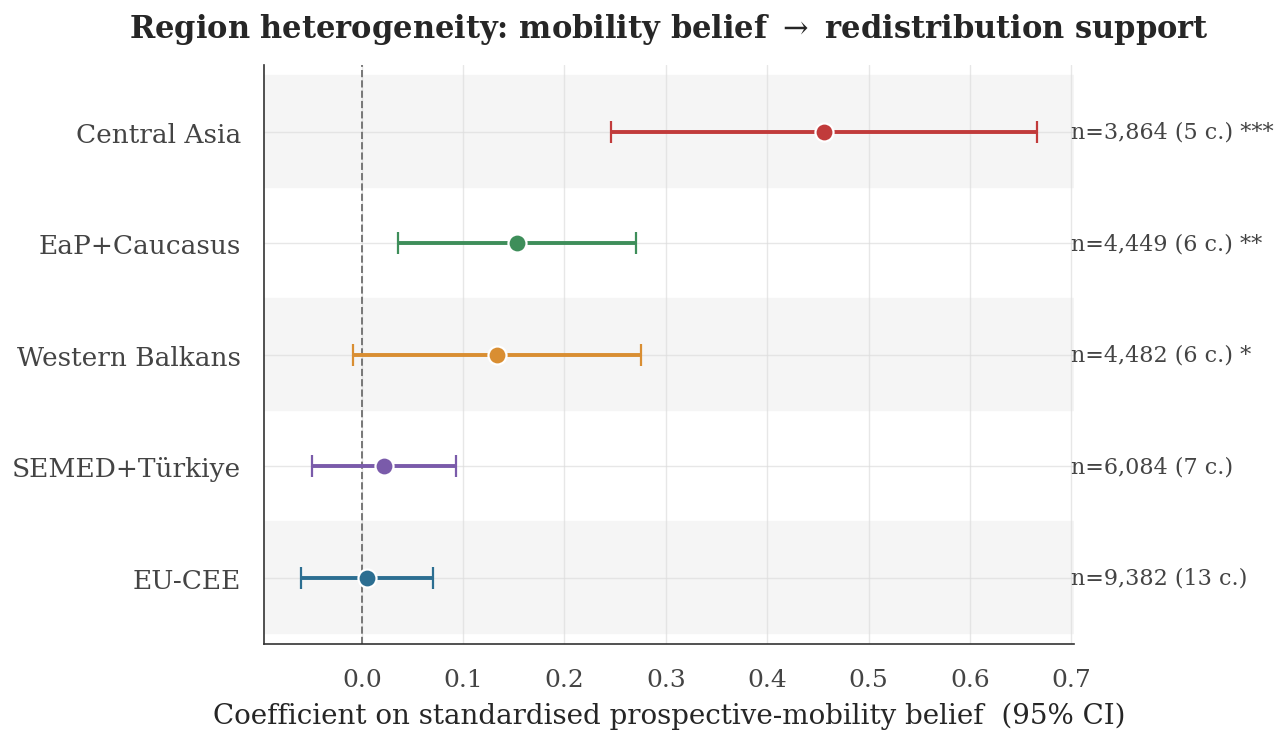
\includegraphics[width=0.74\textwidth]{output/fig_region_coefs.png}
\caption{Coefficient on standardised prospective-mobility belief by LiTS IV region,
with 95\% country-clustered confidence intervals. The cross-region heterogeneity
replaces the binary EU/non-EU framing in \citet{cojocaru2014prospects}.}
\label{fig:region}
\end{figure}

In sum, the data support the dual-channel POUM mechanism of $H_{1}$: ladder-based
self-interest pulls redistribution demand down, attitudinal optimism pulls it up, and
both are conditional on fairness beliefs and institutional region.

\vspace{-6pt}
% =====================================================================
\section{Ethics}

Because no human participants are involved in this study, the ethical risks are
relatively low. However, some of the ethical issues need to be addressed. Firstly,
the study uses secondary analysis of the LiTS IV, which is a publicly available
dataset. The secondary analysis is anonymised, and this study is exempt from
institutional ethics review. The dataset is used strictly for academic purposes.

Another ethical responsibility is confidentiality and privacy. No personal information
is contained in the dataset. Respondents are identified only through unique numbers.
The study does not attempt to re-identify any individual.

Another issue is to represent the results transparently and to interpret them
correctly. The study presents all findings transparently, including null results.
Moreover, as this study design is non-experimental, results are presented as
associations rather than causal effects. As research on how people support
redistribution can affect decisions in the real world, the outcome should not be
misinterpreted. In addition, evidence that mobility beliefs reduce support for
redistribution could be misused for cutting social programmes. The study does not
support any policy. All data sources, software, and literature are cited, and the
analysis is designed to be fully reproducible from the publicly available dataset.
Replication code is openly available (Appendix~C), and the raw microdata are not
redistributed.


\vspace{-6pt}
% =====================================================================
\section{Timeline}
\vspace{-4pt}

\begin{figure}[H]
\centering
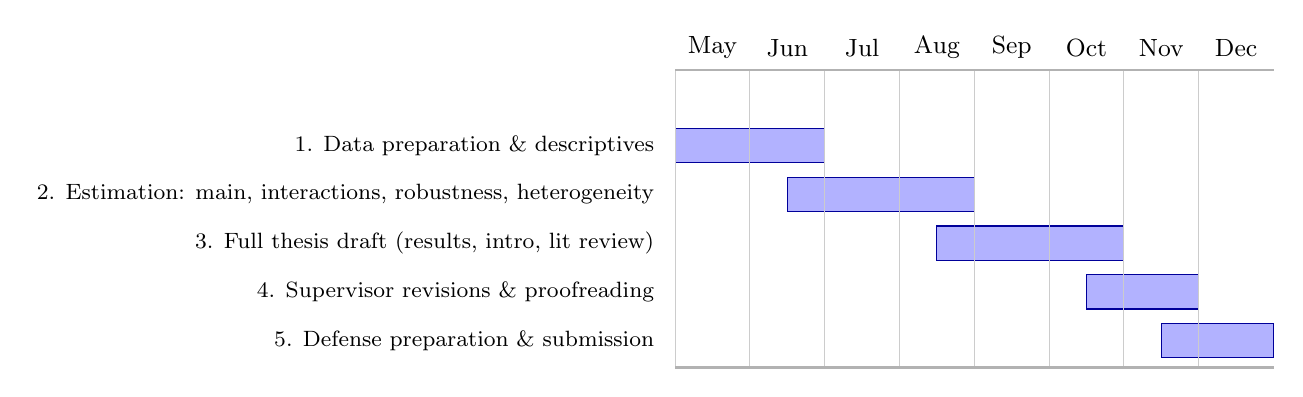
\begin{tikzpicture}[x=0.95cm,y=0.62cm]
% Tasks: (start, length, row, label)
\foreach \start/\len/\row/\lab in {%
  0/2/1/{1. Data preparation \& descriptives},%
  1.5/2.5/2/{2. Estimation: main, interactions, robustness, heterogeneity},%
  3.5/2.5/3/{3. Full thesis draft (results, intro, lit review)},%
  5.5/1.5/4/{4. Supervisor revisions \& proofreading},%
  6.5/1.5/5/{5. Defense preparation \& submission}}{%
  \filldraw[fill=blue!30,draw=blue!60!black]
    (\start,-\row+0.25) rectangle (\start+\len,-\row-0.45);
  \node[anchor=east,font=\footnotesize] at (-0.15,-\row-0.1) {\lab};
}
% Month grid + labels (after bars so labels sit on top)
\foreach \m [count=\i from 0] in {May,Jun,Jul,Aug,Sep,Oct,Nov,Dec}{%
  \draw[gray!40,thin] (\i,0.45) -- (\i,-5.65);
  \node[font=\small] at (\i+0.5,0.9) {\m};
}
\draw[gray!60,thick] (0,0.45) -- (8,0.45);
\draw[gray!60,thick] (0,-5.65) -- (8,-5.65);
\end{tikzpicture}
\caption{Planned timeline (May--December 2026).}
\label{fig:gantt}
\end{figure}

\clearpage
% =====================================================================
\bibliographystyle{plainnat}
\begin{thebibliography}{99}

\bibitem[Abadie et~al.(2023)]{abadie2023should}
Abadie, A., Athey, S., Imbens, G.~W., \& Wooldridge, J.~M. (2023).
\newblock When should you adjust standard errors for clustering?
\newblock \emph{Quarterly Journal of Economics}, 138(1), 1--35.

\bibitem[Alesina \& Angeletos(2005)]{alesina2005fairness}
Alesina, A., \& Angeletos, G.-M. (2005).
\newblock Fairness and redistribution.
\newblock \emph{American Economic Review}, 95(4), 960--980.

\bibitem[Alesina \& Fuchs-Sch\"undeln(2007)]{alesina2007goodbye}
Alesina, A., \& Fuchs-Sch\"undeln, N. (2007).
\newblock Good-bye Lenin (or not?): The effect of communism on people's preferences.
\newblock \emph{American Economic Review}, 97(4), 1507--1528.

\bibitem[Alesina \& La~Ferrara(2005)]{alesina2005preferences}
Alesina, A., \& La~Ferrara, E. (2005).
\newblock Preferences for redistribution in the land of opportunities.
\newblock \emph{Journal of Public Economics}, 89(5--6), 897--931.

\bibitem[Alesina, Stantcheva, \& Teso(2018)]{alesina2018intergenerational}
Alesina, A., Stantcheva, S., \& Teso, E. (2018).
\newblock Intergenerational mobility and preferences for redistribution.
\newblock \emph{American Economic Review}, 108(2), 521--554.

\bibitem[B\'enabou \& Ok(2001)]{benabou2001social}
B\'enabou, R., \& Ok, E.~A. (2001).
\newblock Social mobility and the demand for redistribution: The POUM hypothesis.
\newblock \emph{Quarterly Journal of Economics}, 116(2), 447--487.

\bibitem[B\'enabou \& Tirole(2006)]{benabou2006belief}
B\'enabou, R., \& Tirole, J. (2006).
\newblock Belief in a just world and redistributive politics.
\newblock \emph{Quarterly Journal of Economics}, 121(2), 699--746.

\bibitem[Cameron \& Miller(2015)]{cameron2015practitioner}
Cameron, A.~C., \& Miller, D.~L. (2015).
\newblock A practitioner's guide to cluster-robust inference.
\newblock \emph{Journal of Human Resources}, 50(2), 317--372.

\bibitem[Cantril(1965)]{cantril1965pattern}
Cantril, H. (1965).
\newblock \emph{The Pattern of Human Concerns}.
\newblock Rutgers University Press.

\bibitem[Cojocaru(2014)]{cojocaru2014prospects}
Cojocaru, A. (2014).
\newblock Prospects of upward mobility and preferences for redistribution: Evidence from
the Life in Transition Survey.
\newblock \emph{European Journal of Political Economy}, 34, 300--314.

\bibitem[Deaton(2008)]{deaton2008income}
Deaton, A. (2008).
\newblock Income, health, and well-being around the world: Evidence from the Gallup World
Poll.
\newblock \emph{Journal of Economic Perspectives}, 22(2), 53--72.

\bibitem[EBRD(2024)]{ebrd2024lits}
European Bank for Reconstruction and Development. (2024).
\newblock \emph{Life in Transition Survey IV: A Decade of Surveying Transition.}
\newblock Technical report, EBRD, London.

\bibitem[Giuliano \& Spilimbergo(2014)]{giuliano2014growing}
Giuliano, P., \& Spilimbergo, A. (2014).
\newblock Growing up in a recession.
\newblock \emph{Review of Economic Studies}, 81(2), 787--817.

\bibitem[Hirschman \& Rothschild(1973)]{hirschman1973changing}
Hirschman, A.~O., \& Rothschild, M. (1973).
\newblock The changing tolerance for income inequality in the course of economic
development.
\newblock \emph{Quarterly Journal of Economics}, 87(4), 544--566.

\bibitem[Hoy \& Mager(2021)]{hoy2021relatively}
Hoy, C., \& Mager, F. (2021).
\newblock Why are relatively poor people not more supportive of redistribution? Evidence
from a randomized survey experiment across ten countries.
\newblock \emph{American Economic Journal: Economic Policy}, 13(4), 299--328.

\bibitem[Jaime-Castillo \& Marqu\'es-Perales(2019)]{jaime2019social}
Jaime-Castillo, A.~M., \& Marqu\'es-Perales, I. (2019).
\newblock Social mobility and demand for redistribution in Europe: A comparative
analysis.
\newblock \emph{British Journal of Sociology}, 70(2), 645--670.

\bibitem[Meltzer \& Richard(1981)]{meltzer1981rational}
Meltzer, A.~H., \& Richard, S.~F. (1981).
\newblock A rational theory of the size of government.
\newblock \emph{Journal of Political Economy}, 89(5), 914--927.

\bibitem[Piketty(1995)]{piketty1995social}
Piketty, T. (1995).
\newblock Social mobility and redistributive politics.
\newblock \emph{Quarterly Journal of Economics}, 110(3), 551--584.

\bibitem[Ravallion \& Lokshin(2000)]{ravallion2000wants}
Ravallion, M., \& Lokshin, M. (2000).
\newblock Who wants to redistribute? The tunnel effect in 1990s Russia.
\newblock \emph{Journal of Public Economics}, 76(1), 87--104.

\bibitem[Kuziemko et~al.(2015)]{kuziemko2015elastic}
Kuziemko, I., Norton, M.~I., Saez, E., \& Stantcheva, S. (2015).
\newblock How elastic are preferences for redistribution? Evidence from randomized survey experiments.
\newblock \emph{American Economic Review}, 105(4), 1478--1508.

\bibitem[Karadja, Mollerstrom, \& Seim(2017)]{karadja2017richer}
Karadja, M., Mollerstrom, J., \& Seim, D. (2017).
\newblock Richer (and holier) than thou? The effect of relative-income improvements on demand for redistribution.
\newblock \emph{Review of Economics and Statistics}, 99(2), 201--212.

\bibitem[Roth \& Wohlfart(2018)]{roth2018expected}
Roth, C., \& Wohlfart, J. (2018).
\newblock Experienced inequality and preferences for redistribution.
\newblock \emph{Journal of Public Economics}, 167, 251--262.

\bibitem[Stantcheva(2021)]{stantcheva2021perceptions}
Stantcheva, S. (2021).
\newblock Understanding tax policy: How do people reason?
\newblock \emph{Quarterly Journal of Economics}, 136(4), 2309--2369.

\bibitem[Grosfeld \& Senik(2010)]{grosfeld2010comparing}
Grosfeld, I., \& Senik, C. (2010).
\newblock The emerging aversion to inequality: Evidence from subjective data.
\newblock \emph{Economics of Transition}, 18(1), 1--26.

\bibitem[Wooldridge(2010)]{wooldridge2010econometric}
Wooldridge, J.~M. (2010).
\newblock \emph{Econometric Analysis of Cross Section and Panel Data} (2nd ed.).
\newblock MIT Press.

\end{thebibliography}

\clearpage
% =====================================================================
\appendix
\section*{Appendix A: Variables and Codebook}
\addcontentsline{toc}{section}{Appendix A: Variables and Codebook}

\begin{table}[!ht]
\small
\centering
\caption{LiTS IV variables used in the analysis.}
\label{tab:vars}
\begin{tabularx}{\linewidth}{lXl}
\toprule
\textbf{Variable} & \textbf{LiTS IV item} & \textbf{Coding} \\
\midrule
\textit{Outcomes} & & \\
Redistribution support (DV1) & Q4.01f: ``The gap between the rich and the poor in
[country] should be reduced.'' & 1--5 Likert (pro-redistribution) \\
Willingness to pay (DV2) & Q4.05e: Willingness to pay more taxes for assisting the poor /
reducing inequality. & 1=Yes, 0=No (recoded) \\
\midrule
\textit{Mobility beliefs} & & \\
Retrospective (parents) & Q4.01b: ``I have done better in life than my parents.'' & 1--5 Likert \\
Retrospective (4-year) & Q4.01c: ``My household lives better nowadays than around
4 years ago.'' & 1--5 Likert \\
Prospective (children) & Q4.01e: ``Children who are born now will have a better life
than my generation.'' & 1--5 Likert \\
Current ladder & Q2.35: 10-step wealth ladder, today. & 1--10 \\
Past ladder & Q2.36: 10-step wealth ladder, 4 years ago. & 1--10 \\
Future ladder & Q2.37: 10-step wealth ladder, 4 years from now. & 1--10 \\
Expected ladder mobility & Q2.37 $-$ Q2.35. & $-9$ to $+9$ \\
Realised ladder mobility & Q2.35 $-$ Q2.36. & $-9$ to $+9$ \\
\midrule
\textit{Fairness moderator} & & \\
Effort belief & Q4.06 = 1 (effort/hard work). & 0/1 \\
Injustice belief & Q4.06 $\in\{3,4\}$ (political connections, breaking the law). & 0/1 \\
\midrule
\textit{Controls} & & \\
Female & Roster gender field, indexed by \texttt{rand\_resp\_code}. & 0/1 \\
Age, age$^2$ & Roster age field, indexed by \texttt{rand\_resp\_code}. & years \\
Tertiary education & Q1.09b $\geq 6$. & 0/1 \\
Married & Q1.07b = 2. & 0/1 \\
Urban & \texttt{urbanity} = 1. & 0/1 \\
Log income & $\ln$(Q2.25). & continuous \\
\bottomrule
\end{tabularx}
\end{table}

\clearpage
\section*{Appendix B: Tables}
\addcontentsline{toc}{section}{Appendix B: Tables}

\begin{table}[!ht]
\small
\centering
\caption{Descriptive statistics for the analysis sample (LiTS IV, 37 economies).}
\label{tab:desc}
\begin{tabular}{lrrrrr}
\toprule
Variable & N & Mean & SD & Min & Max \\
\midrule
Redistribution support (1--5) & 35{,}766 & 4.119 & 0.977 & 1 & 5 \\
Willingness to pay (0/1)      & 33{,}456 & 0.496 & 0.500 & 0 & 1 \\
Retrospective: vs.\ parents (1--5)   & 34{,}808 & 3.244 & 1.242 & 1 & 5 \\
Retrospective: 4-year (1--5)         & 35{,}223 & 2.935 & 1.284 & 1 & 5 \\
Prospective: children (1--5)         & 33{,}521 & 3.219 & 1.294 & 1 & 5 \\
Current ladder (1--10)               & 35{,}437 & 4.221 & 1.713 & 1 & 10 \\
Expected ladder mobility ($-9..+9$)  & 31{,}550 & 0.432 & 1.649 & $-9$ & 9 \\
Realised ladder mobility ($-9..+9$)  & 35{,}168 & $-0.273$ & 1.518 & $-9$ & 9 \\
Effort belief (0/1)                  & 34{,}835 & 0.431 & 0.495 & 0 & 1 \\
Injustice belief (0/1)               & 34{,}835 & 0.260 & 0.439 & 0 & 1 \\
Female (0/1)                         & 35{,}766 & 0.591 & 0.492 & 0 & 1 \\
Age (years)                          & 35{,}766 & 47.9  & 17.2  & 18 & 95 \\
Tertiary education (0/1)             & 35{,}766 & 0.264 & 0.441 & 0 & 1 \\
Married (0/1)                        & 35{,}633 & 0.537 & 0.499 & 0 & 1 \\
Urban (0/1)                          & 35{,}766 & 0.603 & 0.489 & 0 & 1 \\
$\ln(\text{income})$                 & 30{,}108 & 8.99  & 2.70  & 0.7 & 19.0 \\
\bottomrule
\end{tabular}
\end{table}

\begin{table}[!ht]
\small
\centering
\caption{Main OLS results: standardised redistribution support on standardised mobility
beliefs, with country fixed effects and clustered standard errors. Each row is a
separate regression, controlling for female, age, age$^2$, tertiary, married, urban,
and $\ln$(income).}
\label{tab:main}
\begin{tabular}{lrrrrr}
\toprule
Mobility variable (z) & N & $\hat\beta$ & SE & $p$ & R$^2$ \\
\midrule
Retrospective: vs.\ parents   & 29{,}361 & $+0.121^{***}$ & 0.023 & $<0.001$ & 0.052 \\
Retrospective: 4-year         & 29{,}663 & $+0.020$       & 0.026 & 0.44     & 0.039 \\
Prospective: children         & 28{,}261 & $+0.098^{***}$ & 0.030 & 0.001    & 0.048 \\
Current ladder                & 29{,}929 & $-0.085^{***}$ & 0.017 & $<0.001$ & 0.045 \\
Expected ladder mobility      & 26{,}863 & $-0.015$       & 0.013 & 0.24     & 0.040 \\
Realised ladder mobility      & 29{,}755 & $-0.049^{***}$ & 0.014 & $<0.001$ & 0.041 \\
\bottomrule
\end{tabular}
\\\footnotesize \emph{Notes.} Country-clustered SEs. $^{*}p<0.10$,
$^{**}p<0.05$, $^{***}p<0.01$.
\end{table}

\begin{table}[!ht]
\small
\centering
\caption{Fairness-belief moderation: interaction between mobility belief and
binary fairness indicator. Reported coefficients are for the interaction term
(\cref{eq:int}). Other rows omitted for brevity.}
\label{tab:int}
\begin{tabular}{llrrrrr}
\toprule
Mobility (z) & Moderator & N & $\hat\beta_{\text{mob}}$ & $\hat\theta$ &
$\hat\pi_{\text{int}}$ & $p_{\text{int}}$ \\
\midrule
Retro: parents     & Effort     & 28{,}780 & $+0.119^{***}$ & $-0.012$       & $+0.002$       & 0.91 \\
Retro: parents     & Injustice  & 28{,}780 & $+0.125^{***}$ & $+0.038$       & $-0.018$       & 0.42 \\
Prospective: kids  & Effort     & 27{,}739 & $+0.069^{**}$  & $-0.012$       & $+0.069^{***}$ & 0.003 \\
Prospective: kids  & Injustice  & 27{,}739 & $+0.121^{***}$ & $+0.027$       & $-0.077^{***}$ & $<0.001$ \\
Expected ladder    & Effort     & 26{,}438 & $-0.020$       & $-0.003$       & $+0.012$       & 0.45 \\
Expected ladder    & Injustice  & 26{,}438 & $-0.008$       & $+0.031$       & $-0.028^{*}$   & 0.10 \\
\bottomrule
\end{tabular}
\\\footnotesize \emph{Notes.} OLS with country fixed effects and country-clustered SEs.
$^{*}p<0.10$, $^{**}p<0.05$, $^{***}p<0.01$.
\end{table}

\begin{table}[!ht]
\small
\centering
\caption{Robustness: linear-probability model on willingness to pay more taxes for
inequality reduction (Q4.05e). Each row is a separate regression with country FE and
clustered SEs.}
\label{tab:wtp}
\begin{tabular}{lrrrrr}
\toprule
Mobility variable (z) & N & $\hat\beta$ & SE & $p$ & R$^2$ \\
\midrule
Retrospective: vs.\ parents & 27{,}726 & $+0.022^{***}$ & 0.005 & $<0.001$ & 0.18 \\
Prospective: children       & 26{,}685 & $+0.025^{***}$ & 0.006 & $<0.001$ & 0.18 \\
Expected ladder mobility    & 25{,}393 & $+0.031^{***}$ & 0.006 & $<0.001$ & 0.19 \\
\bottomrule
\end{tabular}
\\\footnotesize \emph{Notes.} Same controls as in \cref{tab:main}. $^{***}p<0.01$.
\end{table}

\begin{table}[!ht]
\small
\centering
\caption{Population-weighted (WLS) re-estimation of the main specification using
\texttt{weight\_pop} weights. Each row is a separate WLS regression with country fixed
effects and country-clustered SEs.}
\label{tab:weighted}
\begin{tabular}{lrrrr}
\toprule
Mobility variable (z) & N & $\hat\beta$ & SE & $p$ \\
\midrule
Retrospective: vs.\ parents & 29{,}284 & $+0.157^{***}$ & 0.036 & $<0.001$ \\
Retrospective: 4-year       & 29{,}582 & $-0.005$       & 0.054 & 0.93     \\
Prospective: children       & 28{,}198 & $+0.073^{*}$   & 0.039 & 0.06     \\
Current ladder              & 29{,}848 & $-0.052^{**}$  & 0.023 & 0.02     \\
Expected ladder mobility    & 26{,}785 & $-0.026$       & 0.030 & 0.37     \\
Realised ladder mobility    & 29{,}674 & $-0.062^{***}$ & 0.024 & $<0.01$  \\
\bottomrule
\end{tabular}
\\\footnotesize \emph{Notes.} WLS with \texttt{weight\_pop}. $^{*}p<0.10$,
$^{**}p<0.05$, $^{***}p<0.01$.
\end{table}

\begin{table}[!ht]
\small
\centering
\caption{Ordered-logit re-estimation of the redistribution Likert (1--5). Country fixed
effects included. SEs are model-based.}
\label{tab:ologit}
\begin{tabular}{lrrrr}
\toprule
Mobility variable (z) & N & $\hat\beta$ & SE & $p$ \\
\midrule
Retrospective: vs.\ parents   & 29{,}361 & $+0.165^{***}$ & 0.012 & $<0.001$ \\
Prospective: children         & 28{,}261 & $+0.103^{***}$ & 0.013 & $<0.001$ \\
Expected ladder mobility      & 26{,}863 & $-0.039^{***}$ & 0.013 & 0.003    \\
Current ladder                & 29{,}929 & $-0.192^{***}$ & 0.013 & $<0.001$ \\
\bottomrule
\end{tabular}
\\\footnotesize \emph{Notes.} \texttt{statsmodels.OrderedModel} (logit link). Country FE
included as dummies. SEs are model-based, and clustered SEs are not natively available for
this estimator.
\end{table}

\begin{table}[!ht]
\small
\centering
\caption{Joint ``horse-race'' regression with all four mobility variables on the
right-hand side simultaneously. Country FE and country-clustered SEs.
$N=25{,}148$, $R^{2}=0.070$.}
\label{tab:joint}
\begin{tabular}{lrrrl}
\toprule
Mobility variable (z) & $\hat\beta$ & SE & $p$ & Channel \\
\midrule
Retrospective: vs.\ parents     & $+0.126^{***}$ & 0.021 & $<0.001$ & broad-optimism \\
Prospective: children           & $+0.083^{***}$ & 0.028 & 0.003    & broad-optimism \\
Current ladder                  & $-0.128^{***}$ & 0.018 & $<0.001$ & POUM (level) \\
Expected ladder mobility        & $-0.057^{***}$ & 0.012 & $<0.001$ & POUM (expectation) \\
\bottomrule
\end{tabular}
\\\footnotesize \emph{Notes.} Same controls as \cref{tab:main}. The two
ladder-based channels are POUM-consistent. The two attitudinal items are not.
$^{***}p<0.01$.
\end{table}

\begin{table}[!ht]
\small
\centering
\caption{Heterogeneity by current ladder position. Each row is a separate regression on
the indicated sub-sample with prospective-mobility belief on the right-hand side.}
\label{tab:ladder}
\begin{tabular}{lrrrr}
\toprule
Ladder group & N & $\hat\beta$ & SE & $p$ \\
\midrule
Bottom (rungs 1--3) & 9{,}525  & $+0.042^{*}$   & 0.023 & 0.06    \\
Middle (rungs 4--6) & 16{,}471 & $+0.133^{***}$ & 0.036 & $<0.001$\\
Top (rungs 7--10)   & 2{,}165  & $+0.274^{***}$ & 0.070 & $<0.001$\\
\bottomrule
\end{tabular}
\\\footnotesize \emph{Notes.} Mobility variable: \texttt{mob\_prospect\_kids\_z}.
\end{table}

\begin{table}[!ht]
\small
\centering
\caption{Heterogeneity by age cohort (born before vs.\ from 1980).}
\label{tab:cohort}
\begin{tabular}{llrrrr}
\toprule
Cohort & Mobility variable (z) & N & $\hat\beta$ & SE & $p$ \\
\midrule
Born $<$1980    & Prospective: children      & 16{,}377 & $+0.089^{***}$ & 0.027 & 0.002 \\
Born $<$1980    & Expected ladder mobility   & 15{,}395 & $-0.028^{**}$  & 0.013 & 0.03  \\
Born $\geq$1980 & Prospective: children      & 11{,}884 & $+0.113^{***}$ & 0.038 & 0.004 \\
Born $\geq$1980 & Expected ladder mobility   & 11{,}468 & $+0.003$       & 0.017 & 0.87  \\
\bottomrule
\end{tabular}
\\\footnotesize \emph{Notes.} Country FE and country-clustered SEs.
\end{table}

\begin{table}[!ht]
\small
\centering
\caption{Five-region split. DV: standardised redistribution
support. Mobility variable: \texttt{mob\_prospect\_kids\_z}.}
\label{tab:regions}
\begin{tabular}{lrrrrr}
\toprule
Region & N (obs.) & Countries & $\hat\beta$ & SE & $p$ \\
\midrule
EU-CEE              & 9{,}382 & 13 & $+0.005$       & 0.034 & 0.88   \\
Western Balkans     & 4{,}482 & 6  & $+0.133^{*}$   & 0.072 & 0.07   \\
EaP+Caucasus        & 4{,}449 & 6  & $+0.153^{**}$  & 0.060 & 0.01   \\
Central Asia        & 3{,}864 & 5  & $+0.456^{***}$ & 0.107 & $<0.001$\\
SEMED+Türkiye       & 6{,}084 & 7  & $+0.022$       & 0.037 & 0.55   \\
\bottomrule
\end{tabular}
\\\footnotesize \emph{Notes.} Country FE within each region and country-clustered SEs.
\end{table}

\clearpage
\section*{Appendix C: Replication Code}
\addcontentsline{toc}{section}{Appendix C: Replication Code}

All code, tables, and figures are openly available at:
\begin{center}
\url{https://github.com/DovudAsadov/mobility-beliefs-redistribution}
\end{center}

\noindent The repository contains:
\begin{itemize}[leftmargin=18pt,itemsep=2pt]
    \item \href{https://github.com/DovudAsadov/mobility-beliefs-redistribution/blob/main/analysis/build_dataset.py}{\texttt{analysis/build\_dataset.py}}: reads the LiTS IV \texttt{.dta} file and constructs the cleaned analysis dataset.
    \item \href{https://github.com/DovudAsadov/mobility-beliefs-redistribution/blob/main/analysis/regressions.py}{\texttt{analysis/regressions.py}}: estimates Equations~\eqref{eq:base} and \eqref{eq:int} plus all robustness and
    heterogeneity checks, and writes \crefrange{tab:desc}{tab:regions} and
    \crefrange{fig:country}{fig:region} into
    \href{https://github.com/DovudAsadov/mobility-beliefs-redistribution/tree/main/output}{\texttt{output/}}.
    \item \href{https://github.com/DovudAsadov/mobility-beliefs-redistribution/blob/main/paper.tex}{\texttt{paper.tex}}:
    the LaTeX source of this proposal.
    \item \href{https://github.com/DovudAsadov/mobility-beliefs-redistribution/blob/main/README.md}{\texttt{README.md}}:
    step-by-step reproduction instructions and environment setup.
\end{itemize}

\noindent The raw LiTS IV microdata is licensed by the EBRD and not redistributed in the
repository. It can be downloaded directly from the
\href{https://www.ebrd.com/what-we-do/economic-research-and-data/data/lits.html}{EBRD LiTS data portal}.

\clearpage
% =====================================================================
\section*{Appendix D: Declaration of AI Use}
\addcontentsline{toc}{section}{Appendix D: Declaration of AI Use}

In line with the course submission rules, I declare that generative AI tools
(Anthropic's Claude, accessed through Claude Code) were used in the preparation of this
proposal in the following capacities:

\begin{itemize}[leftmargin=18pt,itemsep=2pt]
    \item \emph{Drafting assistance and copy-editing.} AI was used to refine prose,
    tighten word counts to the rubric limits, and surface formatting issues in the
    LaTeX source.
    \item \emph{Code review and figure design.} AI assisted in reviewing the Python
    analysis scripts (data cleaning, regressions, plots) and suggested visual
    improvements (ISO-3 labels, region colour coding, confidence-interval bands,
    \texttt{adjustText} for label placement).
    \item \emph{Structural feedback.} AI was used to audit the proposal against the
    course rubric (word limits, section coverage) and to suggest tighter framings of
    objectives, research questions, and hypotheses.
\end{itemize}

\noindent AI was \emph{not} used to generate the empirical findings, choose the
research question, conduct the literature search, or determine the substantive
conclusions. All econometric specifications, theoretical framings, and interpretations
are my own, and I take full responsibility for the content of this proposal.

\end{document}
